% =========================================================
%  Relatório — Atividade Avaliativa 1
%  Curadoria de Datasets e Inferência Básica com LLMs
%  Equipe 3 — Domínio Jurídico
% =========================================================
\documentclass[12pt,a4paper]{article}

% -------------------- Idioma e fontes --------------------
\usepackage[T1]{fontenc}
\usepackage[utf8]{inputenc}
\usepackage[brazil]{babel}

% -------------------- Layout -----------------------------
\usepackage[a4paper,margin=2.5cm]{geometry}
\usepackage{setspace}
\onehalfspacing

% -------------------- Utilidades -------------------------
\usepackage{graphicx}
\usepackage{float}
\usepackage{booktabs}
\usepackage{tabularx}
\usepackage{multirow}
\usepackage{enumitem}
\usepackage{parskip}
\usepackage{hyperref}
\usepackage{url}
\usepackage{amsmath}

% -------------------- Links ------------------------------
\usepackage{hyperref}
\hypersetup{
  colorlinks=true,
  linkcolor=blue!60!black,
  urlcolor=blue!60!black,
  citecolor=blue!60!black
}

% -------------------- Código (Python) --------------------
\usepackage{xcolor}
\usepackage{listings}

\definecolor{pybg}{RGB}{248,248,248}
\definecolor{pyframe}{RGB}{220,220,220}
\definecolor{pyblue}{RGB}{32,64,154}
\definecolor{pystring}{RGB}{163,21,21}
\definecolor{pycomment}{RGB}{120,120,120}

\lstdefinestyle{pythonstyle}{
  language=Python,
  basicstyle=\ttfamily\small,
  keywordstyle=\color{pyblue}\bfseries,
  stringstyle=\color{pystring},
  commentstyle=\color{pycomment}\itshape,
  showstringspaces=false,
  columns=fullflexible,
  backgroundcolor=\color{pybg},
  frame=single,
  rulecolor=\color{pyframe},
  frameround=ffff,
  breaklines=true,
  tabsize=2,
  numbersep=8pt,
  numbers=left,
  numberstyle=\tiny\color{pycomment}
}

\lstdefinestyle{bashstyle}{
  language=bash,
  basicstyle=\ttfamily\small,
  backgroundcolor=\color{pybg},
  frame=single,
  rulecolor=\color{pyframe},
  frameround=ffff,
  breaklines=true,
  numbers=none
}

% -------------------- Metadados --------------------------
\title{%
  \vspace{-1cm}
  \large\textbf{Universidade Federal de Sergipe}\\[0.3cm]
  \normalsize Departamento de Computação\\
  Tópicos Avançados em Engenharia de Software e Sistemas de Informação I\\[1cm]
  \Large\textbf{Atividade Avaliativa 1}\\[0.3cm]
  \large Curadoria de Datasets e Inferência Básica com LLMs\\[0.3cm]
  \normalsize Equipe 3: Domínio Jurídico
}
\author{
  Reinan Gabriel dos Santos Souza \\
  Fernanda Mirely Barbosa Souza \\
  Éricles dos Santos Cunha \\
  Mikaela de Andrade Lima \\
  Victor Leonardo Mascarenhas Soares Horta
}
\date{Abril de 2026}

% =========================================================
\begin{document}
\maketitle
\thispagestyle{empty}

% ----- Informações de acesso em destaque -----
\begin{center}
  \fbox{\parbox{0.85\textwidth}{\centering
    \textbf{Vídeo demonstrativo:}\\
    \url{https://youtu.be/lcOxhH8N3Bo}
  }}
\end{center}

\vspace{0.5cm}
\newpage

\tableofcontents
\newpage

% =========================================================
\section{Introdução}
% =========================================================

Este documento apresenta os resultados da atividade avaliativa 1 da disciplina Tópicos Avançados em Engenharia de Software e Sistemas de Informação I, ministrada na Universidade Federal de Sergipe (UFS), semestre 2026.1.

A atividade consiste na curadoria de datasets jurídicos e na realização de inferência básica utilizando Modelos de Linguagem (LLMs), com foco em questões do Exame da OAB (Ordem dos Advogados do Brasil). Embora a execução das tarefas de curadoria e análise seja individual, a entrega e consolidação dos resultados são feitas em equipe.

O presente relatório documenta as contribuições da \textbf{Equipe 3 (Jurídica)}. Cada membro da equipe ficou responsável por um lote específico de questões, e suas contribuições individuais são detalhadas na Seção~\ref{sec:contribuicoes}.

% =========================================================
\section{Contribuições individuais}
\label{sec:contribuicoes}
% =========================================================

Esta seção detalha as contribuições de cada membro da equipe na execução da atividade.

% ---------------------------------------------------------
\subsection{Reinan Gabriel dos Santos Souza}
% ---------------------------------------------------------

Toda a implementação do pipeline, desde a curadoria das questões até a geração dos gráficos de avaliação, está disponível no repositório público no GitHub\footnote{\url{https://github.com/reinanhs/Topicos_Avancados_2026_1_Equipe_JUD_3_atividade1}}. O repositório segue a abordagem \textit{Docs-as-Code}, com documentação técnica versionada. A partir dele é possível acessar a documentação web e navegar pelos artefatos para visualizar os resultados obtidos.

\subsubsection{Escolha e justificativa dos modelos}

A seleção dos modelos foi condicionada pelo hardware disponível, especificamente uma GPU NVIDIA GeForce GTX 1050 com apenas 4~GB de VRAM dedicada. Essa restrição limitou a escolha a LLMs compactos, com até aproximadamente 3 bilhões de parâmetros, em versões quantizadas que não ultrapassassem 2~GB de armazenamento.

Foram selecionados três modelos de organizações distintas, todos executados localmente via Ollama, a saber, o \textbf{Gemma 2 2B}, o \textbf{Llama 3.2 3B} e o \textbf{Qwen 2.5 3B}. A escolha priorizou três critérios, compatibilidade com o hardware disponível, diversidade de desenvolvedores para evitar viés arquitetural e suporte ao idioma português, requisito essencial para o domínio jurídico brasileiro.

\subsubsection{Resultados da avaliação exata}

A Tabela~\ref{tab:reinan-exata} apresenta o desempenho dos três modelos nas 122 questões objetivas do lote atribuído, avaliados por meio de Acurácia, Precisão, Recall e F1-Score. O \textbf{gemma2:2b} obteve a maior acurácia (0,4344), seguido pelo \textbf{qwen2.5:3b} (0,4180) e \textbf{llama3.2:3b} (0,3607). Nenhum modelo ultrapassou 50\%, resultado esperado considerando o tamanho reduzido dos modelos e a complexidade inerente às questões da OAB.

\begin{table}[H]
\centering
\caption{Avaliação exata do desempenho dos modelos em questões objetivas}
\label{tab:reinan-exata}
\begin{tabular}{lcccc}
\toprule
\textbf{Modelo} & \textbf{Acurácia} & \textbf{Precisão} & \textbf{Recall} & \textbf{F1} \\
\midrule
gemma2:2b   & 0,4344 & 0,4322 & 0,4448 & 0,4101 \\
llama3.2:3b & 0,3607 & 0,3519 & 0,3563 & 0,3473 \\
qwen2.5:3b  & 0,4180 & 0,3609 & 0,3405 & 0,3337 \\
\bottomrule
\end{tabular}
\end{table}

A Figura~\ref{fig:reinan-barras-exatas} permite visualizar essa comparação de forma mais direta. Observa-se que o \textbf{gemma2:2b} mantém valores ligeiramente superiores em todas as métricas, enquanto o \textbf{llama3.2:3b} fica consistentemente abaixo dos demais. A Figura~\ref{fig:reinan-radar-exatas} complementa essa análise com um gráfico radar, no qual o \textbf{gemma2:2b} apresenta o polígono mais simétrico e amplo, indicando o perfil mais equilibrado entre os três modelos.

\begin{figure}[H]
\centering
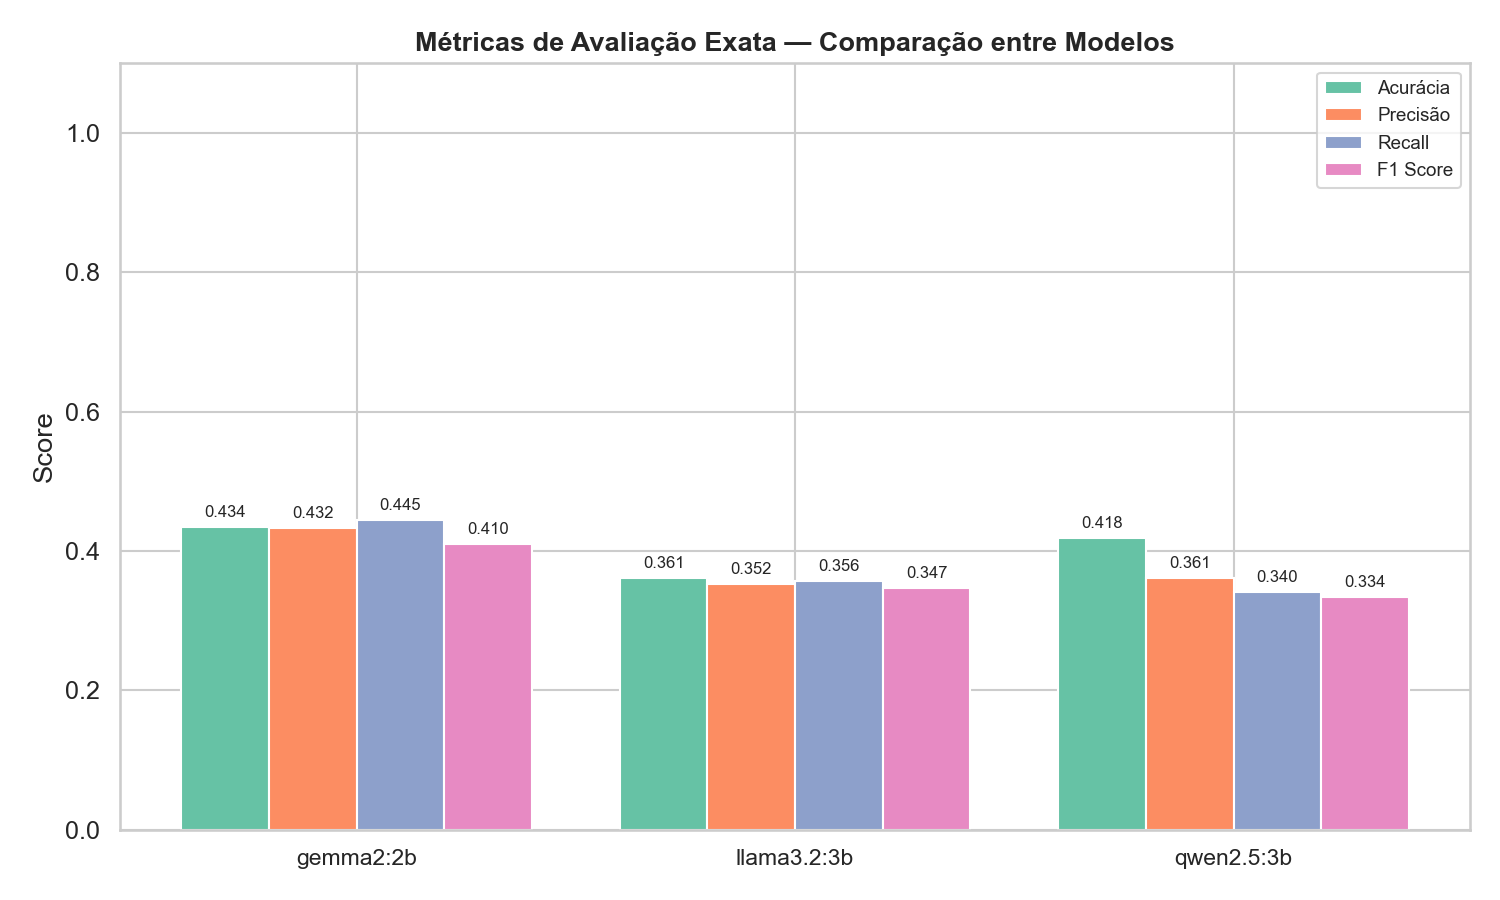
\includegraphics[width=0.85\textwidth]{images/reinan/01_barras_metricas_exatas.png}
\caption{Métricas de avaliação exata na comparação entre modelos}
\label{fig:reinan-barras-exatas}
\end{figure}

\begin{figure}[H]
\centering
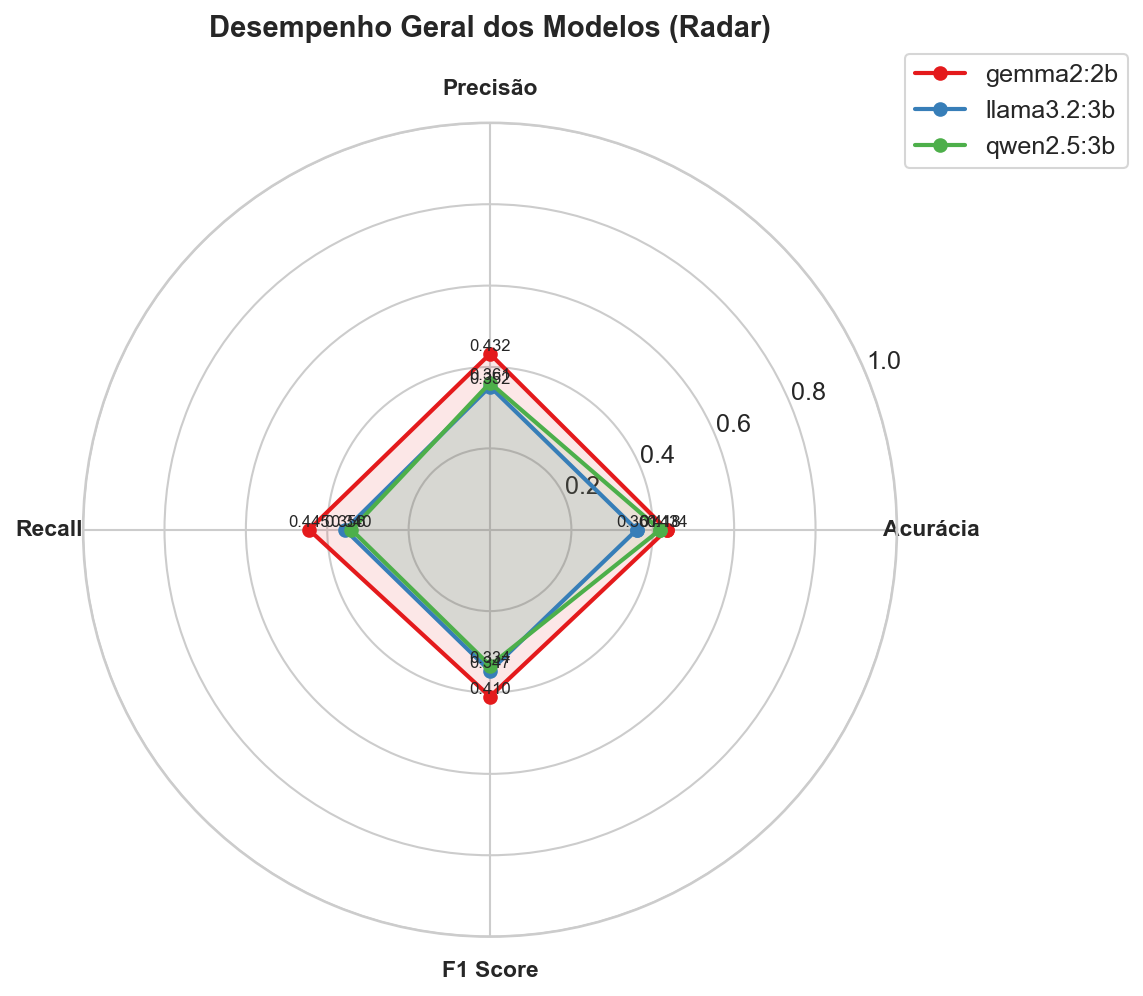
\includegraphics[width=0.55\textwidth]{images/reinan/02_radar_metricas_exatas.png}
\caption{Desempenho geral dos modelos em gráfico radar}
\label{fig:reinan-radar-exatas}
\end{figure}

\subsubsection{Resultados da avaliação cruzada}

Para as 12 questões dissertativas, que não possuem gabarito oficial, a avaliação foi conduzida de duas formas: comparação entre as respostas dos próprios modelos e comparação com a guideline de referência fornecida pelo dataset. A Tabela~\ref{tab:reinan-cross} apresenta as métricas de similaridade entre os pares de modelos, enquanto a Tabela~\ref{tab:reinan-guideline} mostra a aderência de cada modelo à guideline.

\begin{table}[H]
\centering
\caption{Avaliação cruzada de similaridade entre pares de modelos}
\label{tab:reinan-cross}
\small
\setlength{\tabcolsep}{4pt}
\begin{tabular}{lccccc}
\toprule
\textbf{Par de modelos} & \textbf{BLEU} & \textbf{ROUGE-1} & \textbf{ROUGE-2} & \textbf{ROUGE-L} & \textbf{BERTScore F1} \\
\midrule
gemma2:2b vs llama3.2:3b  & 0,1205 & 0,4575 & 0,1789 & 0,2459 & 0,7319 \\
gemma2:2b vs qwen2.5:3b   & 0,1011 & 0,4741 & 0,1734 & 0,2256 & 0,7394 \\
llama3.2:3b vs qwen2.5:3b & 0,1025 & 0,4473 & 0,1664 & 0,2320 & 0,7323 \\
\bottomrule
\end{tabular}
\end{table}

\begin{table}[H]
\centering
\caption{Aderência dos modelos à guideline de referência.}
\label{tab:reinan-guideline}
\small
\setlength{\tabcolsep}{4pt}
\begin{tabular}{lccccc}
\toprule
\textbf{Modelo vs Guideline} & \textbf{BLEU} & \textbf{ROUGE-1} & \textbf{ROUGE-2} & \textbf{ROUGE-L} & \textbf{BERTScore F1} \\
\midrule
gemma2:2b vs guideline   & 0,0216 & 0,1534 & 0,0585 & 0,1126 & 0,6569 \\
llama3.2:3b vs guideline & 0,0215 & 0,1600 & 0,0571 & 0,1113 & 0,6632 \\
qwen2.5:3b vs guideline  & 0,0172 & 0,1260 & 0,0447 & 0,0910 & 0,6513 \\
\bottomrule
\end{tabular}
\end{table}

Os modelos apresentam concordância semântica razoável entre si, com BERTScore F1 acima de 0,73 em todos os pares, apesar da baixa sobreposição lexical (BLEU $\approx$ 0,10--0,12). Já a similaridade com a guideline é consideravelmente menor (BERTScore F1 em torno de 0,65), indicando que, embora os modelos concordem entre si, suas respostas se distanciam do padrão de referência esperado.

A Figura~\ref{fig:reinan-heatmap} ilustra essa diferença por meio de um heatmap de similaridade semântica. As células entre modelos apresentam tons mais intensos (maior similaridade), enquanto as comparações com a guideline aparecem em tons mais claros.

\begin{figure}[H]
\centering
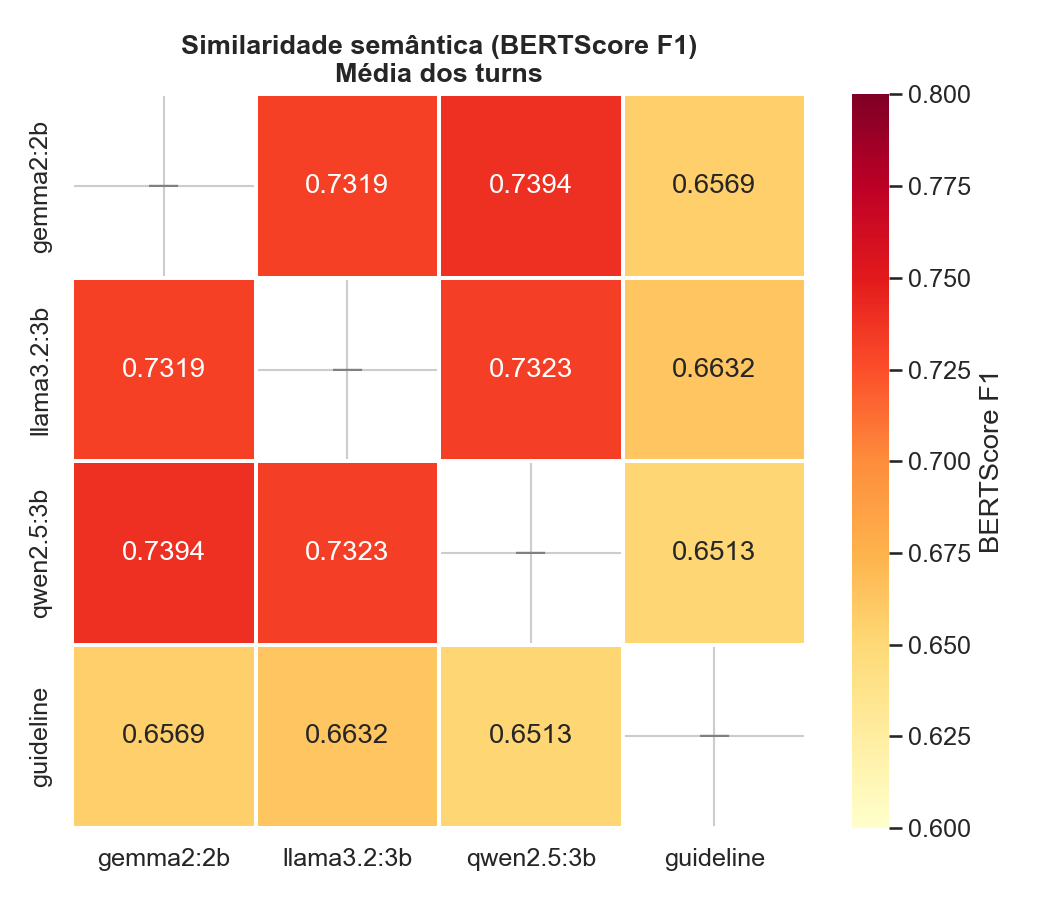
\includegraphics[width=0.65\textwidth]{images/reinan/01_heatmap_bertscore.png}
\caption{Heatmap de similaridade semântica entre modelos e guideline.}
\label{fig:reinan-heatmap}
\end{figure}

A Figura~\ref{fig:reinan-barras-modelos} detalha todas as métricas de similaridade entre os pares de modelos. O BERTScore F1 é consistentemente a métrica mais elevada, enquanto o BLEU permanece baixo, resultado esperado, pois o BERTScore captura a semântica contextual, ao passo que o BLEU depende da correspondência exata de n-gramas.

\begin{figure}[H]
\centering
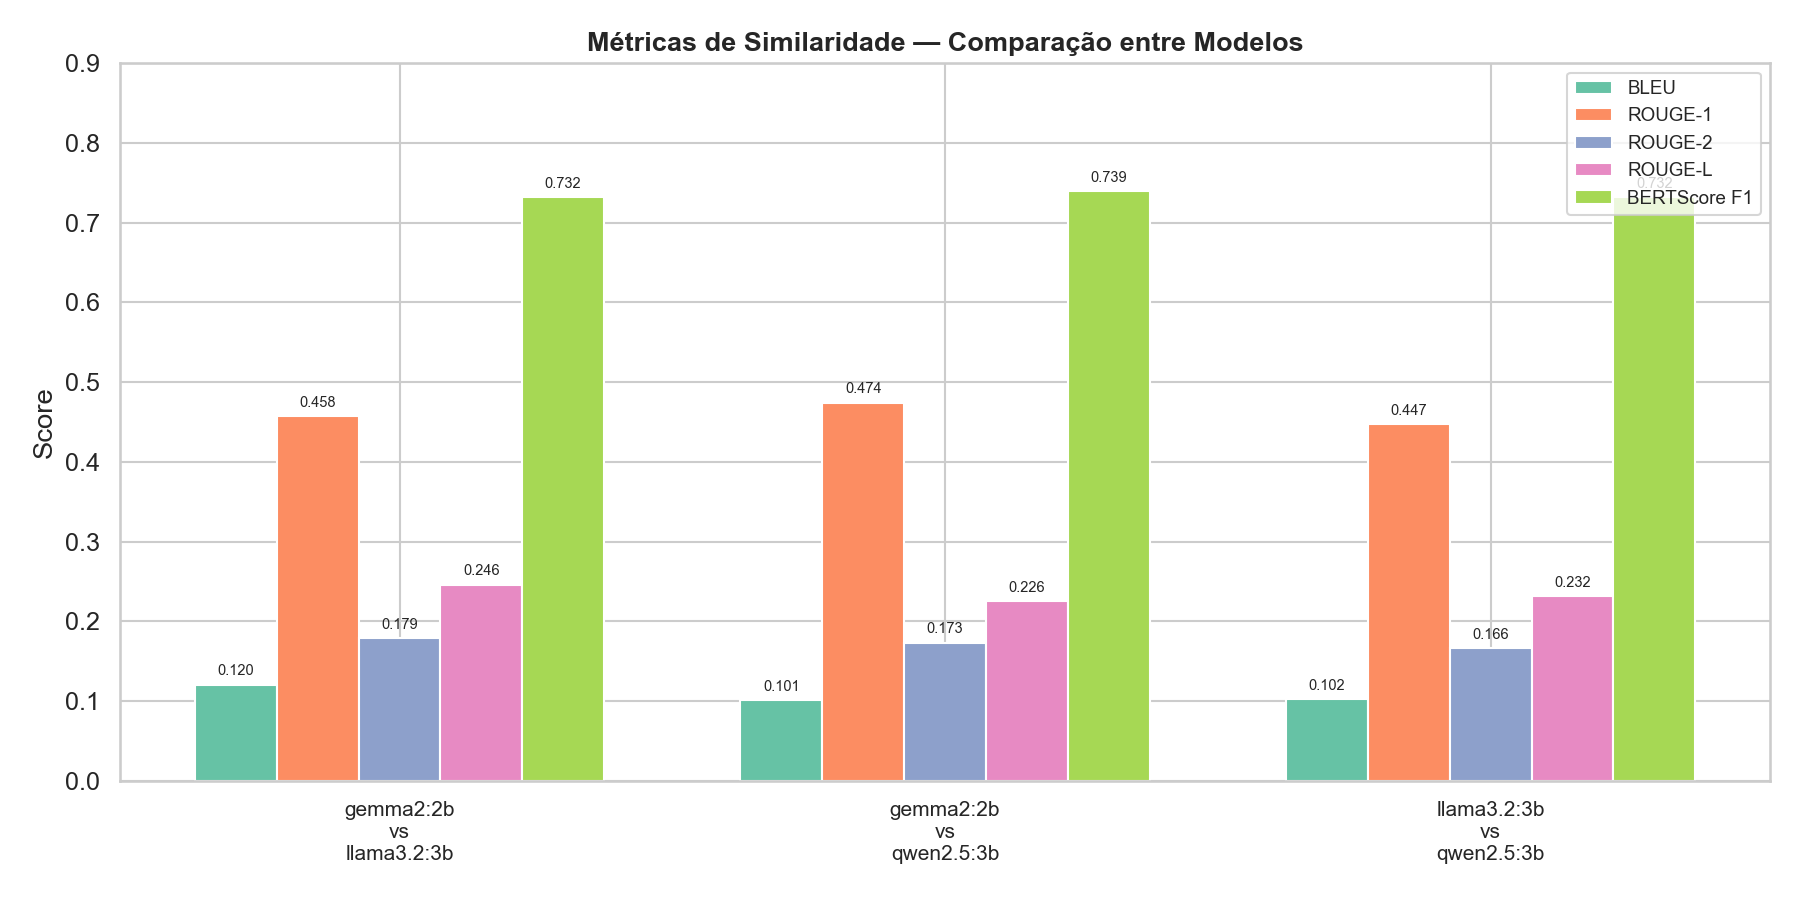
\includegraphics[width=0.65\textwidth]{images/reinan/02_barras_modelo_vs_modelo.png}
\caption{Comparação entre pares de modelos com métricas de similaridade}
\label{fig:reinan-barras-modelos}
\end{figure}

A Figura~\ref{fig:reinan-barras-guideline} apresenta a aderência de cada modelo à guideline. Os valores baixos de BLEU e ROUGE confirmam que os modelos não reproduzem literalmente o texto de referência, embora o BERTScore em torno de 0,65 sugira certa proximidade semântica.

\begin{figure}[H]
\centering
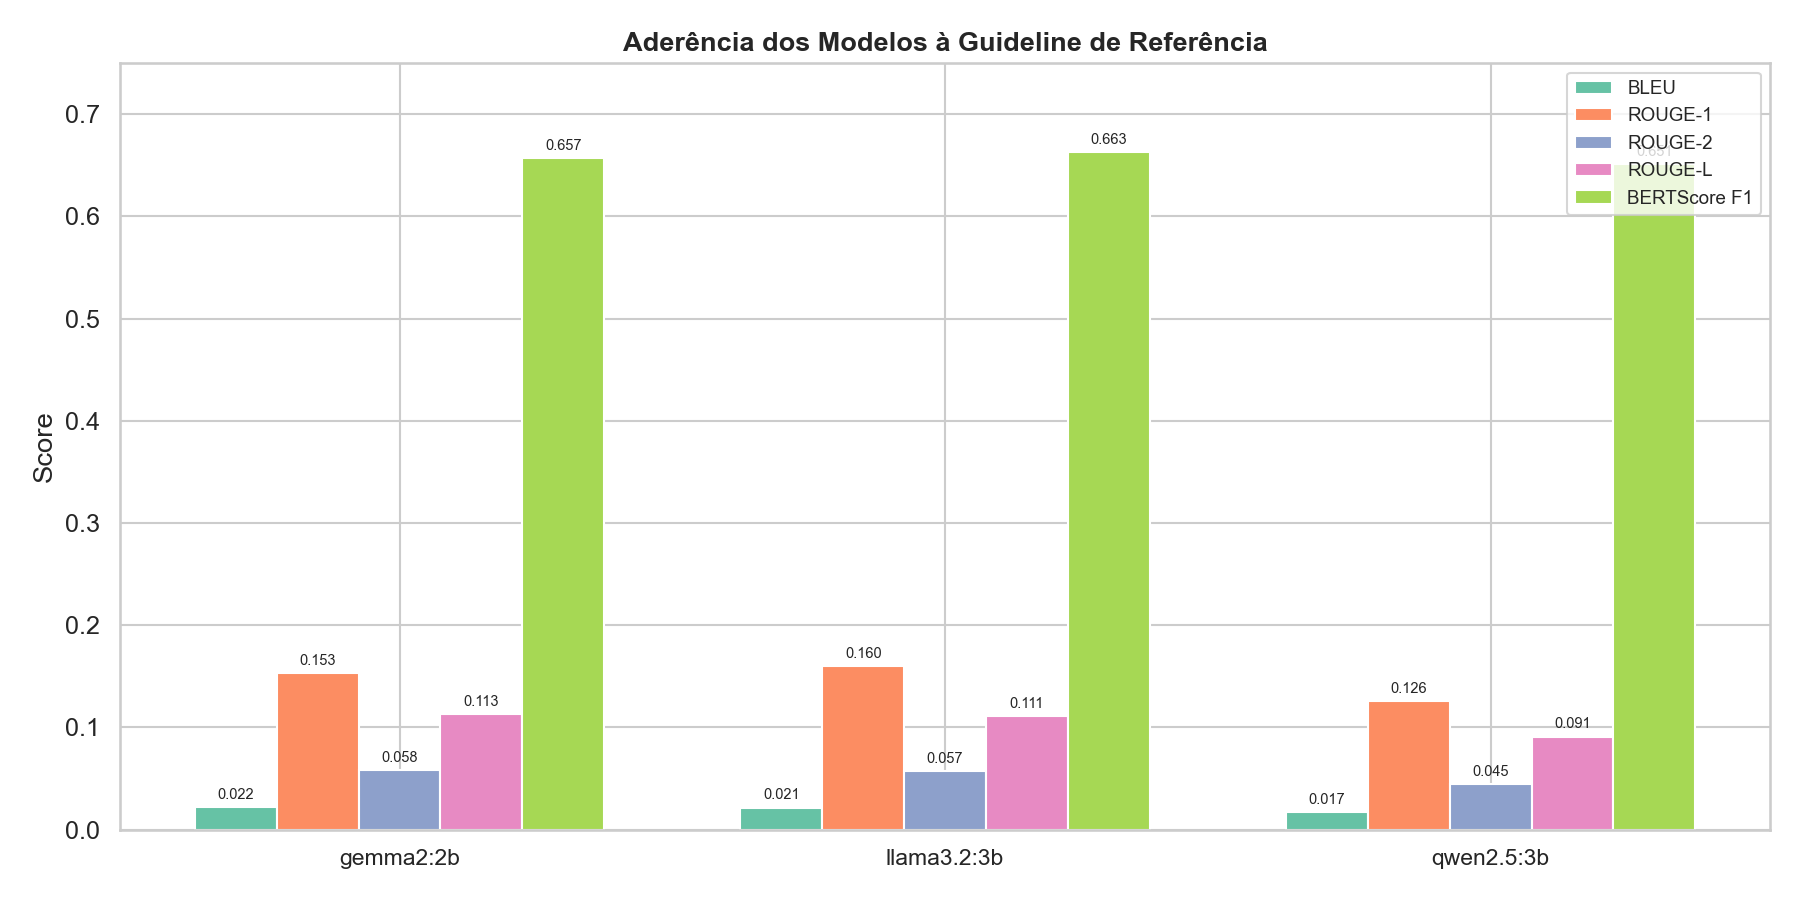
\includegraphics[width=0.85\textwidth]{images/reinan/03_barras_modelo_vs_guideline.png}
\caption{Aderência dos modelos à guideline de referência.}
\label{fig:reinan-barras-guideline}
\end{figure}

A Figura~\ref{fig:reinan-radar-guideline} complementa essa análise com gráficos radar individuais. Todos os modelos apresentam um padrão semelhante: alta concentração no eixo do BERTScore F1 e valores baixos nas demais métricas, reforçando a diferença entre similaridade lexical e semântica.

\begin{figure}[H]
\centering
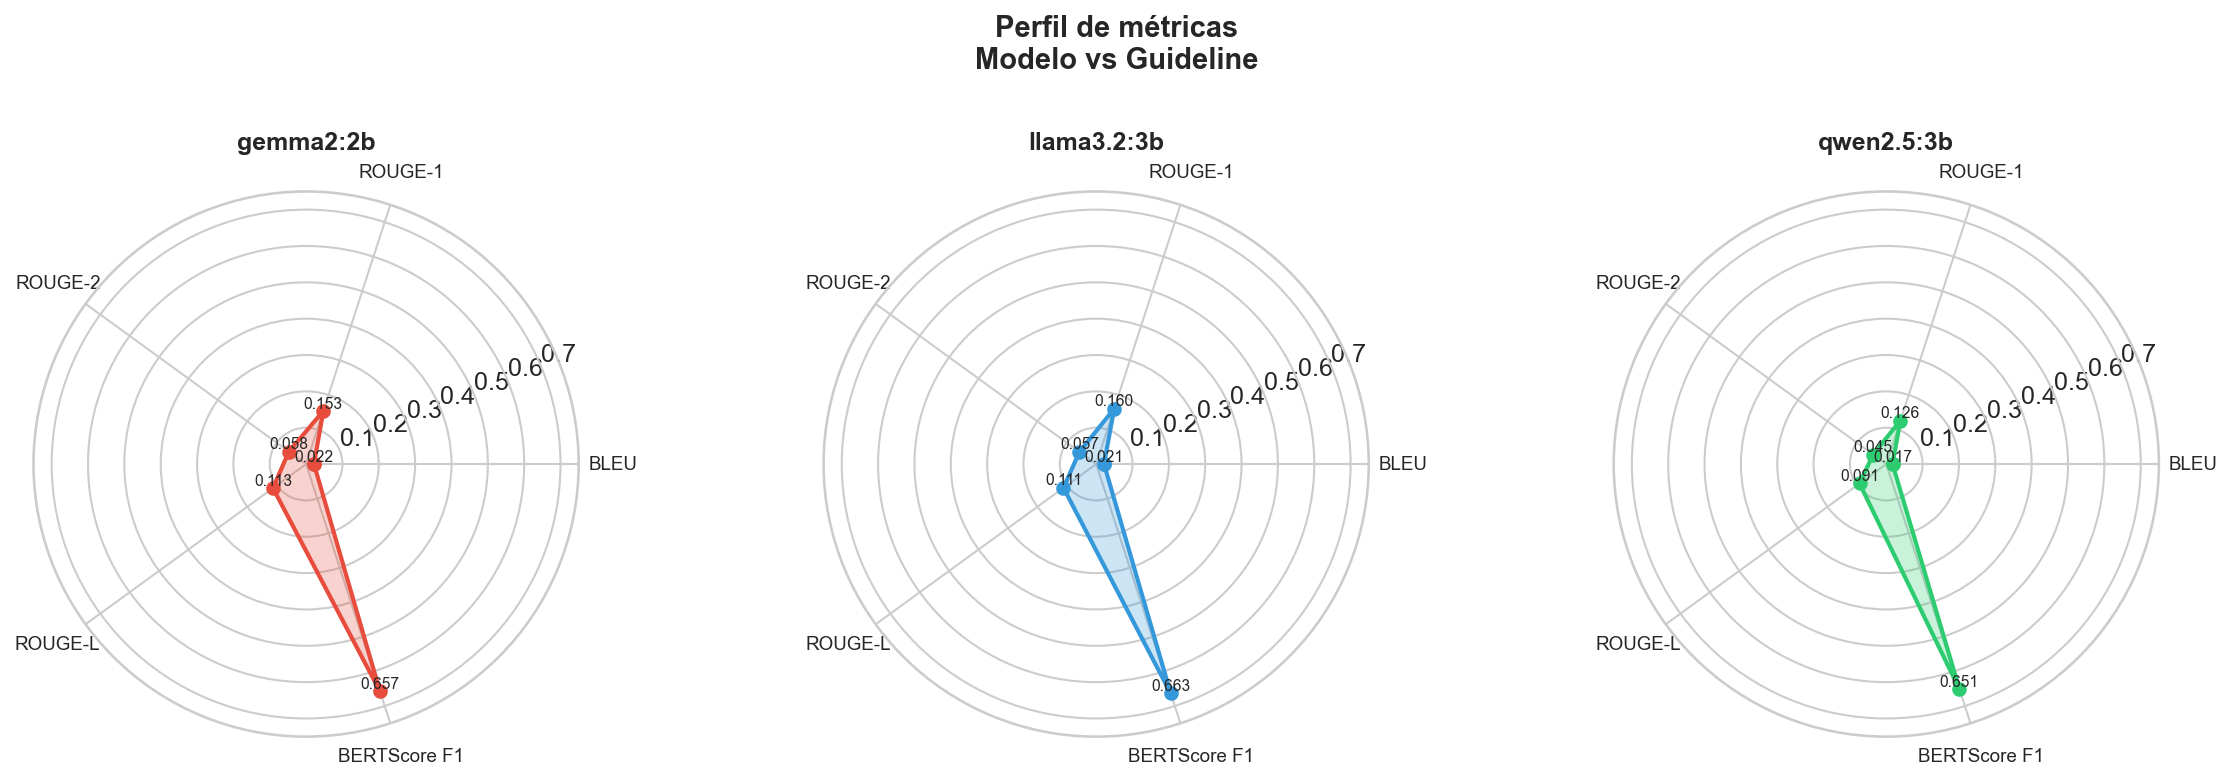
\includegraphics[width=1.0\textwidth]{images/reinan/04_radar_modelo_vs_guideline.png}
\caption{Perfil de métricas por modelo em relação à guideline.}
\label{fig:reinan-radar-guideline}
\end{figure}

A Figura~\ref{fig:reinan-turns} desagrega o BERTScore F1 por turn. O Turn~1 tende a apresentar scores ligeiramente superiores ao Turn~2 em praticamente todos os pares, o que pode indicar que a segunda parte das questões exige respostas mais específicas, nas quais os modelos divergem mais.

\begin{figure}[H]
\centering
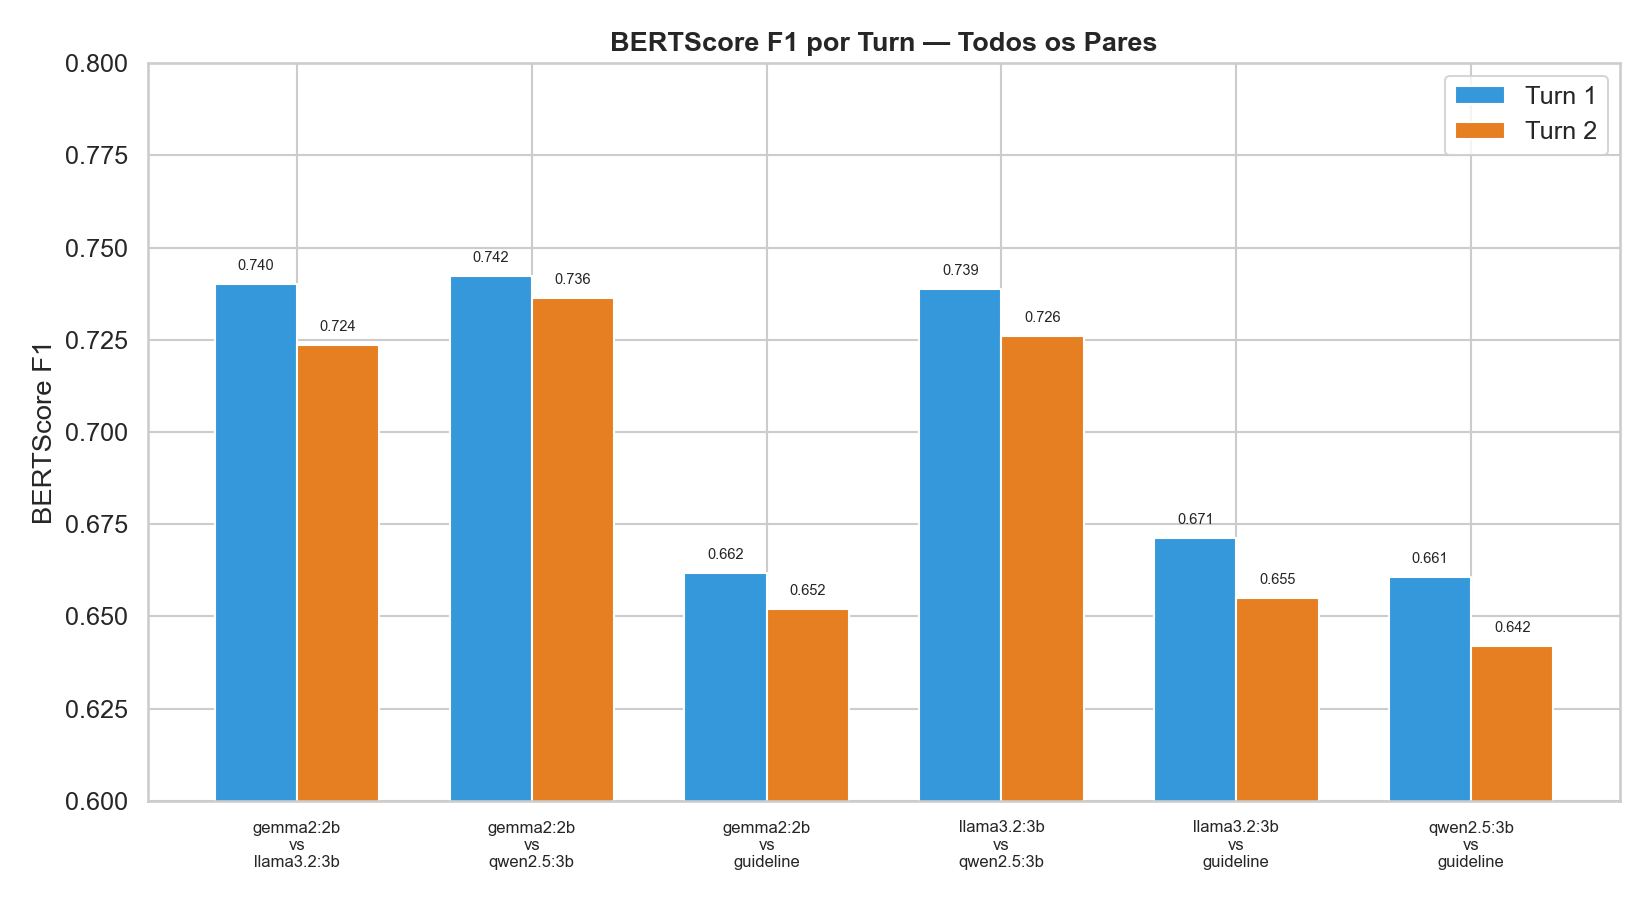
\includegraphics[width=0.85\textwidth]{images/reinan/05_turn1_vs_turn2_bertscore.png}
\caption{Distribuição do BERTScore F1 por turno para todos os pares}
\label{fig:reinan-turns}
\end{figure}

\subsubsection{Resultados da avaliação com modelo juiz}

Além das métricas automáticas de similaridade, um modelo juiz (GPT-4o-mini) foi utilizado para avaliar qualitativamente as respostas dissertativas. A Tabela~\ref{tab:reinan-judge} apresenta os scores médios atribuídos a cada modelo.

\begin{table}[H]
\centering
\caption{Score médio atribuído pelo modelo juiz GPT-4o-mini.}
\label{tab:reinan-judge}
\begin{tabular}{lc}
\toprule
\textbf{Modelo} & \textbf{Score Médio} \\
\midrule
qwen2.5:3b  & 0,189 \\
llama3.2:3b & 0,139 \\
gemma2:2b   & 0,120 \\
\bottomrule
\end{tabular}
\end{table}

A Figura~\ref{fig:reinan-judge-medio} ilustra essa classificação. Os valores baixos de todos os modelos refletem a dificuldade geral de LLMs compactos diante de questões jurídicas dissertativas que exigem fundamentação técnica aprofundada.

\begin{figure}[H]
\centering
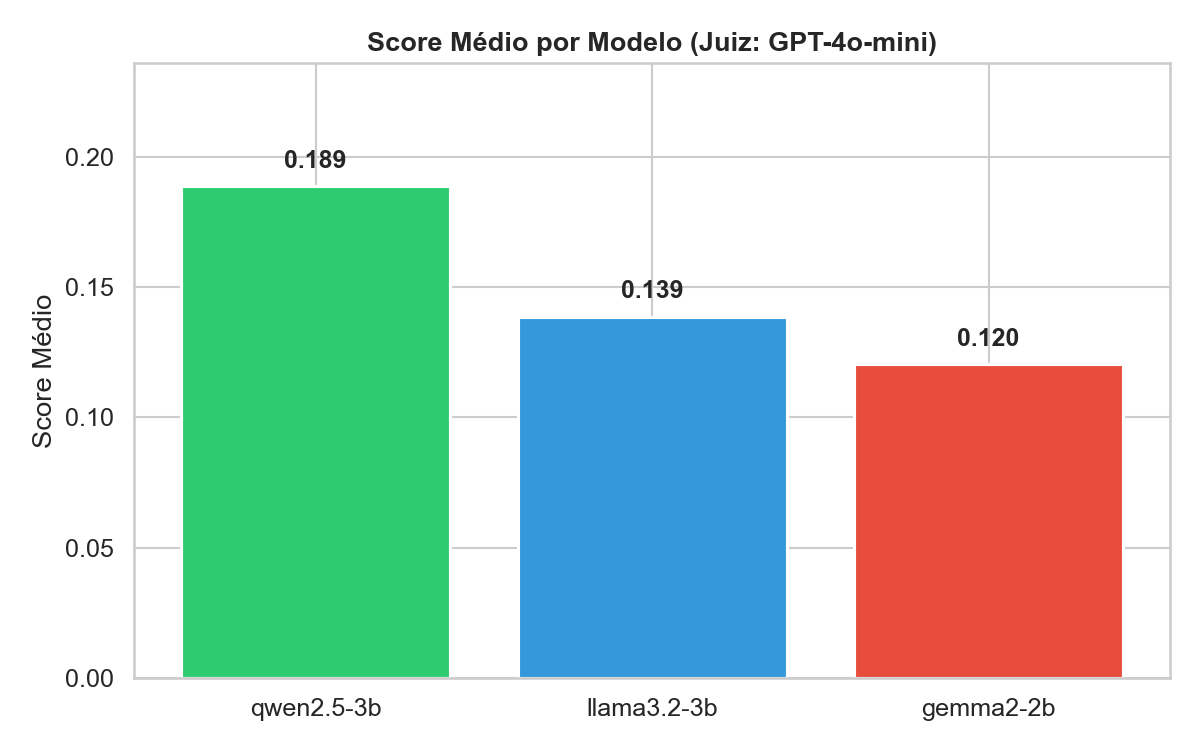
\includegraphics[width=0.45\textwidth]{images/reinan/06_judgment_score_medio.png}
\caption{Score médio por modelo.}
\label{fig:reinan-judge-medio}
\end{figure}

A Figura~\ref{fig:reinan-judge-turn} ilustra que a desagregação por \textit{turn} evidencia comportamentos distintos entre os modelos. O \textbf{llama3.2:3b} apresenta um aumento expressivo do Turn~1 (0,083) para o Turn~2 (0,205), enquanto o \textbf{qwen2.5:3b} exibe comportamento oposto, com redução no segundo \textit{turn}. Esse resultado sugere diferenças na capacidade de aprofundamento das respostas entre os modelos.

\begin{figure}[H]
\centering
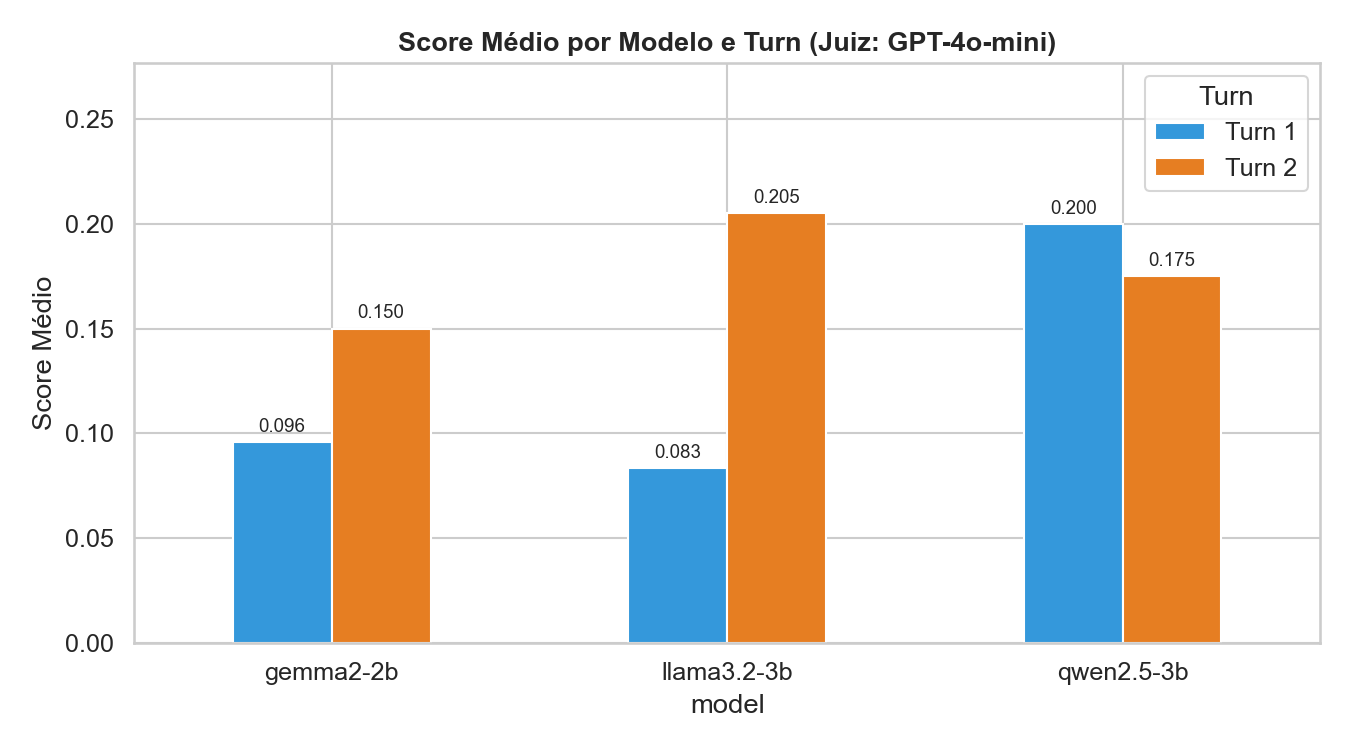
\includegraphics[width=0.65\textwidth]{images/reinan/07_judgment_score_por_turn.png}
\caption{Score do juiz por modelo e turn.}
\label{fig:reinan-judge-turn}
\end{figure}

O heatmap da Figura~\ref{fig:reinan-heatmap-questoes} detalha os scores por questão individual. Questões de direito administrativo obtiveram melhor desempenho geral, enquanto questões de direito do trabalho foram as mais difíceis para todos os modelos. Nota-se também que nenhum modelo domina todas as questões, evidenciando comportamentos complementares entre eles.

\begin{figure}[H]
\centering
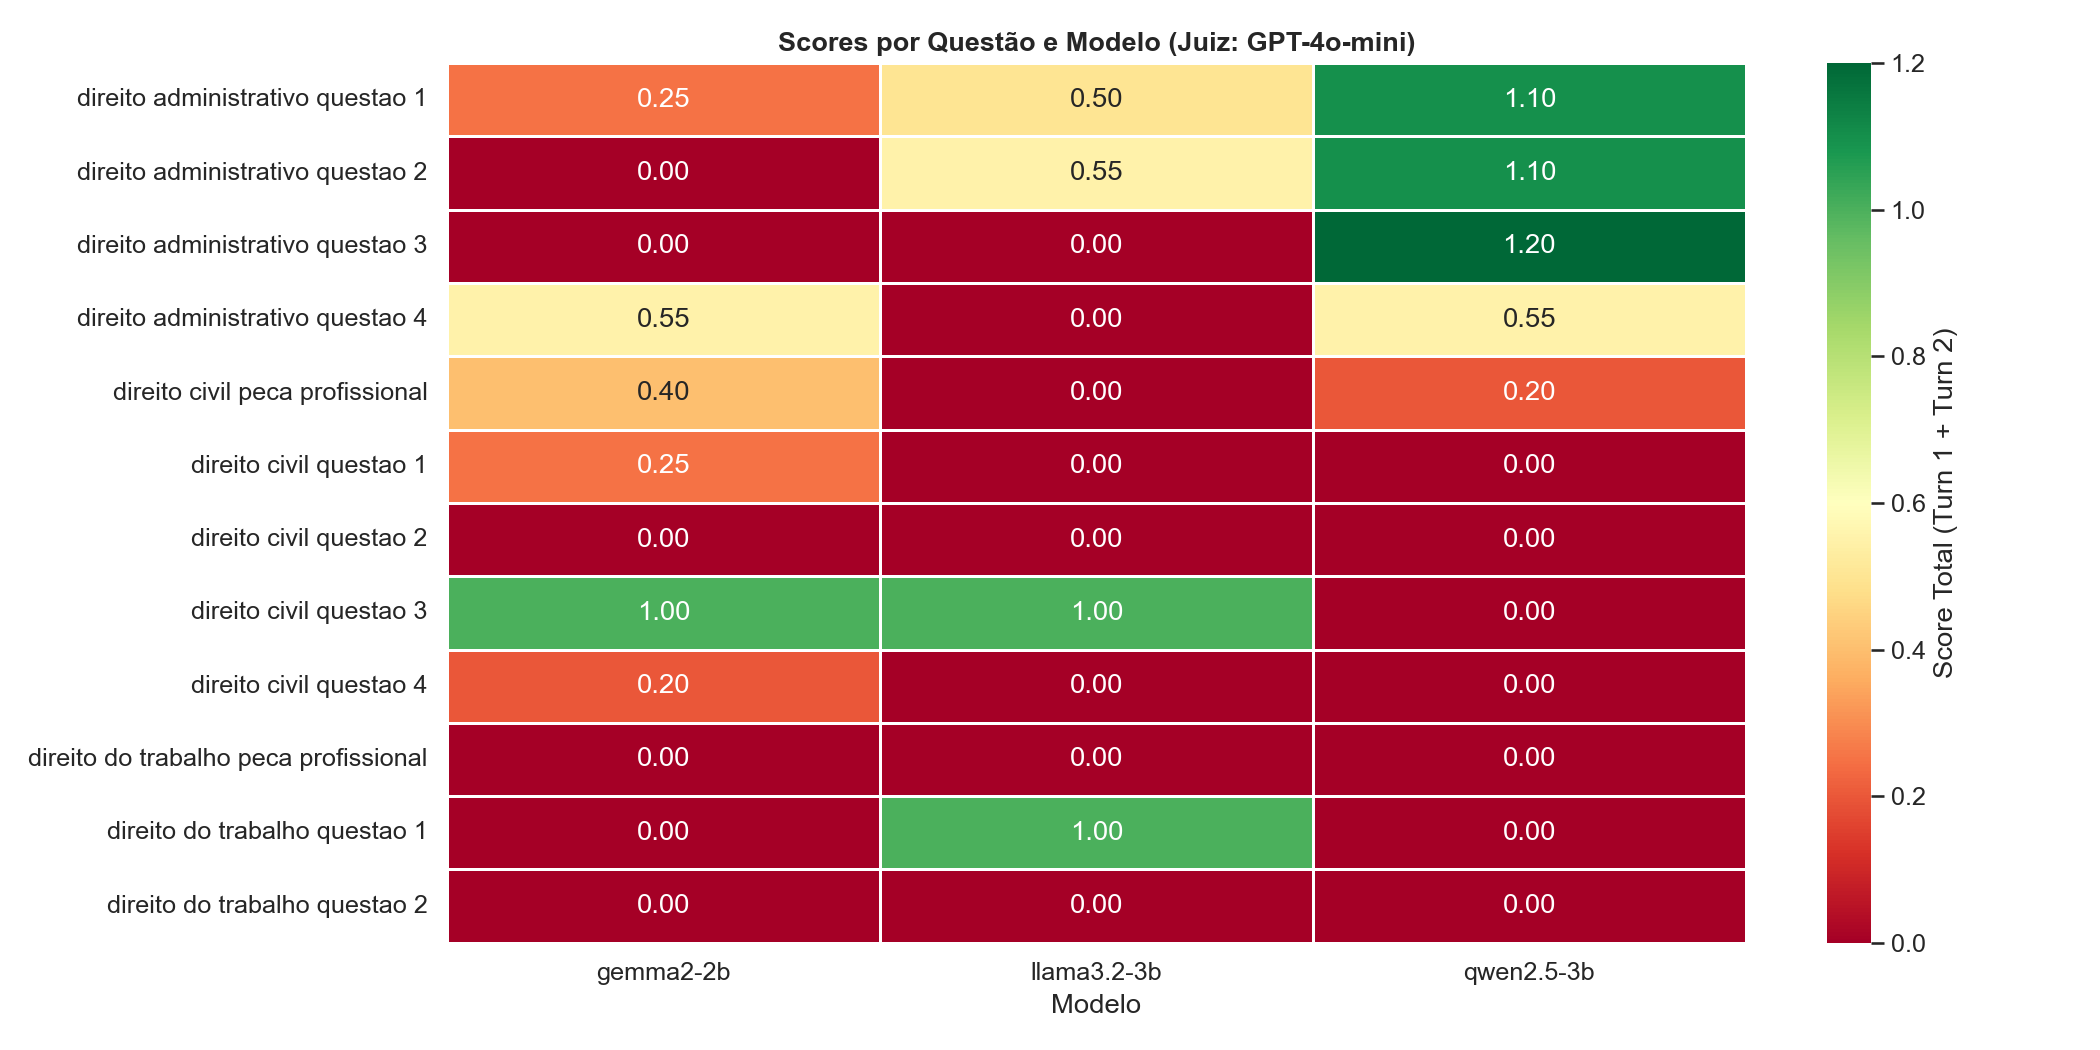
\includegraphics[width=0.95\textwidth]{images/reinan/09_judgment_heatmap_questoes.png}
\caption{Scores do juiz por questão e modelo.}
\label{fig:reinan-heatmap-questoes}
\end{figure}


% ---------------------------------------------------------
\subsection{Fernanda Mirely Barbosa Souza}
% ---------------------------------------------------------

\textbf{Questões atribuídas:} J1: 141--152 | J2: 1477--1599

A implementação completa do pipeline de dados e inferência — abrangendo as etapas de curadoria de questões da OAB, pré-processamento, execução de inferência via LLMs e geração de métricas de avaliação — encontra-se disponível em repositório público no GitHub\footnote{\url{https://github.com/safira1344/Topicos_Avancados_2026_1_Equipe_JUD_3_atividade1}}.



% TODO: Adicionar contribuições individuais

% ---------------------------------------------------------
\subsection{Éricles dos Santos Cunha}
% ---------------------------------------------------------

\textbf{Questões atribuídas:} J1: 153--164 | J2: 1600--1722

A implementação completa do pipeline de dados e inferência — abrangendo as etapas de curadoria de questões da OAB, pré-processamento, execução de inferência via LLMs e geração de métricas de avaliação — encontra-se disponível em repositório público no GitHub\footnote{\url{https://github.com/Ericles-Porty/Topicos_Avancados_2026_1_Equipe_JUD_3_atividade1}}. O repositório segue a abordagem \textit{Docs-as-Code}, integrando documentação técnica e código-fonte sob controle de versão.


\subsubsection{Escolha e justificativa dos modelos}

Os experimentos de inferência foram conduzidos em ambiente local, sob o sistema operacional \textit{Windows} 11. A infraestrutura computacional utilizada foi composta por um processador Intel Core i5 de 13ª geração, 32 GB de memória RAM e uma unidade de processamento gráfico NVIDIA GeForce RTX 3050, com 6,0 GB de memória dedicada (VRAM). A execução padronizada dos modelos foi realizada por meio da ferramenta Ollama, responsável pelo gerenciamento local das requisições e dos pesos das redes neurais, garantindo maior controle e reprodutibilidade dos experimentos.

Foram utilizados o \textbf{Llama 3.2 (3B)}, o \textbf{Gemma 2 (2B)} e o \textbf{Qwen 2.5 (3B)}. Esta escolha fundamentou-se na diversidade de arquitetura, possibilitando a comparação de diferentes metodologias de pré-treinamento e alinhamento em um mesmo domínio jurídico. Por fim, a localização linguística foi um critério determinante, visto que todos os modelos possuem suporte nativo ao idioma português, requisito mandatório para o processamento das questões do Exame da OAB, enquanto a disponibilidade no ecossistema Ollama assegurou a consistência do pipeline e a reprodutibilidade dos resultados.

\subsubsection{Resultados das questões objetivas}

A Tabela~\ref{tab:ericles-exata} apresenta as métricas de classificação obtidas pelos três modelos no conjunto de 122 questões de múltipla escolha. O \textbf{qwen2.5:3b} alcançou o melhor resultado em todos os indicadores, com acurácia de 50,41\% e F1-Score de 0,4742, sendo o único modelo a ultrapassar a marca de 50\% de acerto. O \textbf{llama3.2:3b} ficou em segundo lugar (46,34\%), enquanto o \textbf{gemma2:2b} teve o menor aproveitamento (40,65\%). Apesar de o qwen2.5:3b ter superado os demais, o desempenho geral dos três modelos permanece limitado, o que é esperado para LLMs com menos de 4 bilhões de parâmetros diante da complexidade das questões da OAB.

\begin{table}[H]
\centering
\caption{Métricas de classificação dos modelos nas questões objetivas}
\label{tab:ericles-exata}
\begin{tabular}{lcccc}
\toprule
\textbf{Modelo} & \textbf{Acurácia} & \textbf{Precisão} & \textbf{Recall} & \textbf{F1} \\
\midrule
llama3.2:3b & 0,4634 & 0,4096 & 0,3662 & 0,3632 \\
gemma2:2b   & 0,4065 & 0,4124 & 0,3979 & 0,3884 \\
qwen2.5:3b  & 0,5041 & 0,5250 & 0,4903 & 0,4742 \\
\bottomrule
\end{tabular}
\end{table}

A Figura~\ref{fig:ericles-multipla-escolha} permite visualizar essas métricas de forma direta, evidenciando a vantagem do qwen2.5:3b sobre os demais.

\begin{figure}[H]
\centering
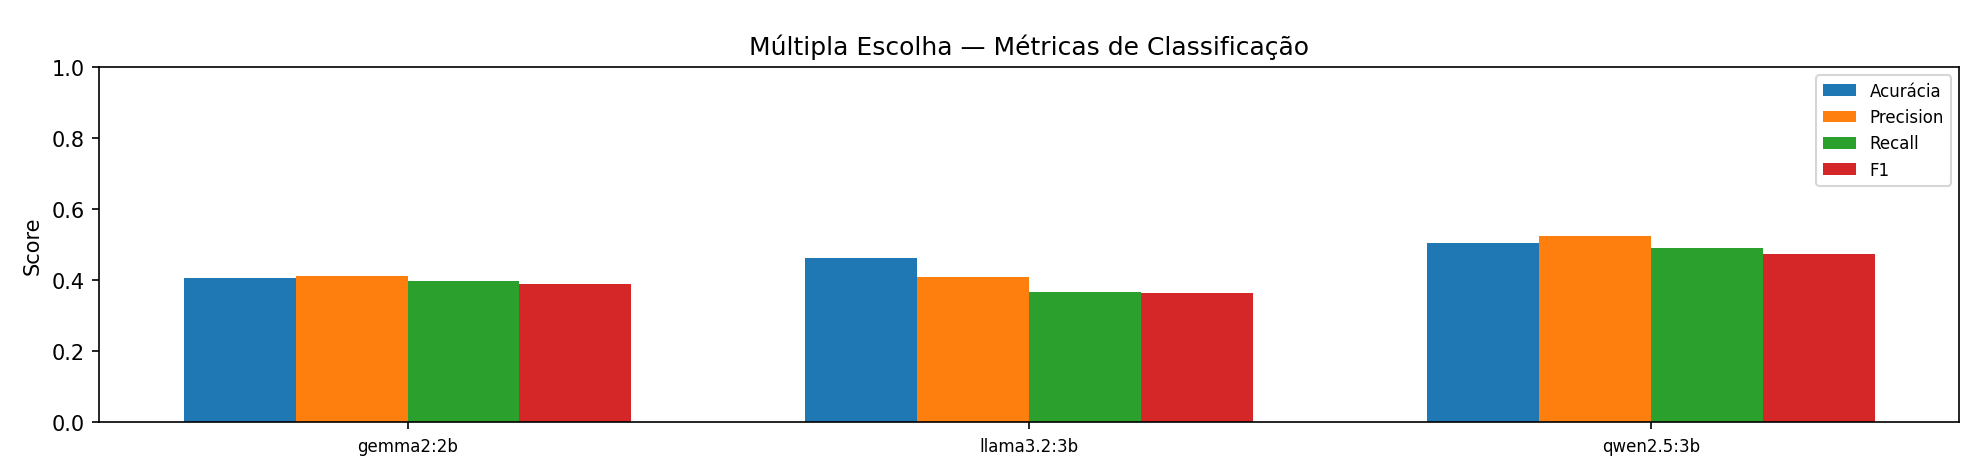
\includegraphics[width=0.85\textwidth]{images/ericles/multipla-escolha-metricas-classificacao.png}
\caption{Métricas de classificação dos modelos nas questões de múltipla escolha}
\label{fig:ericles-multipla-escolha}
\end{figure}

\subsubsection{Consistência entre modelos nas questões abertas}

Para avaliar o grau de concordância entre os modelos nas 12 questões dissertativas, foram calculadas métricas de similaridade textual e semântica entre cada par. A Tabela~\ref{tab:ericles-cross} apresenta os resultados.

\begin{table}[H]
\centering
\caption{Métricas de similaridade entre pares de modelos nas questões abertas}
\label{tab:ericles-cross}
\small
\setlength{\tabcolsep}{4pt}
\begin{tabular}{lccccc}
\toprule
\textbf{Par de modelos} & \textbf{BLEU} & \textbf{ROUGE-1} & \textbf{ROUGE-2} & \textbf{ROUGE-L} & \textbf{BERTScore F1} \\
\midrule
llama3.2:3b vs gemma2:2b  & 0,1550 & 0,4997 & 0,2249 & 0,2651 & 0,7568 \\
llama3.2:3b vs qwen2.5:3b & 0,1288 & 0,4796 & 0,2081 & 0,2405 & 0,7534 \\
gemma2:2b vs qwen2.5:3b   & 0,1145 & 0,5003 & 0,1855 & 0,2222 & 0,7502 \\
\bottomrule
\end{tabular}
\end{table}

Os três pares mantêm BERTScore F1 acima de 0,75, o que indica que, do ponto de vista semântico, os modelos transmitem ideias parecidas mesmo utilizando vocabulários distintos. As métricas lexicais confirmam essa diferença de forma: o BLEU fica entre 0,11 e 0,16 e o ROUGE-L não passa de 0,27, mostrando que a sobreposição literal de termos é baixa. Esse comportamento é natural em respostas jurídicas abertas, onde não existe uma formulação canônica esperada. O par llama3.2:3b--gemma2:2b apresenta os valores mais altos em quase todas as métricas, sugerindo que esses dois modelos produzem respostas mais próximas entre si do que em relação ao qwen2.5:3b. A Figura~\ref{fig:ericles-cross-model} ilustra essa comparação.

\begin{figure}[H]
\centering
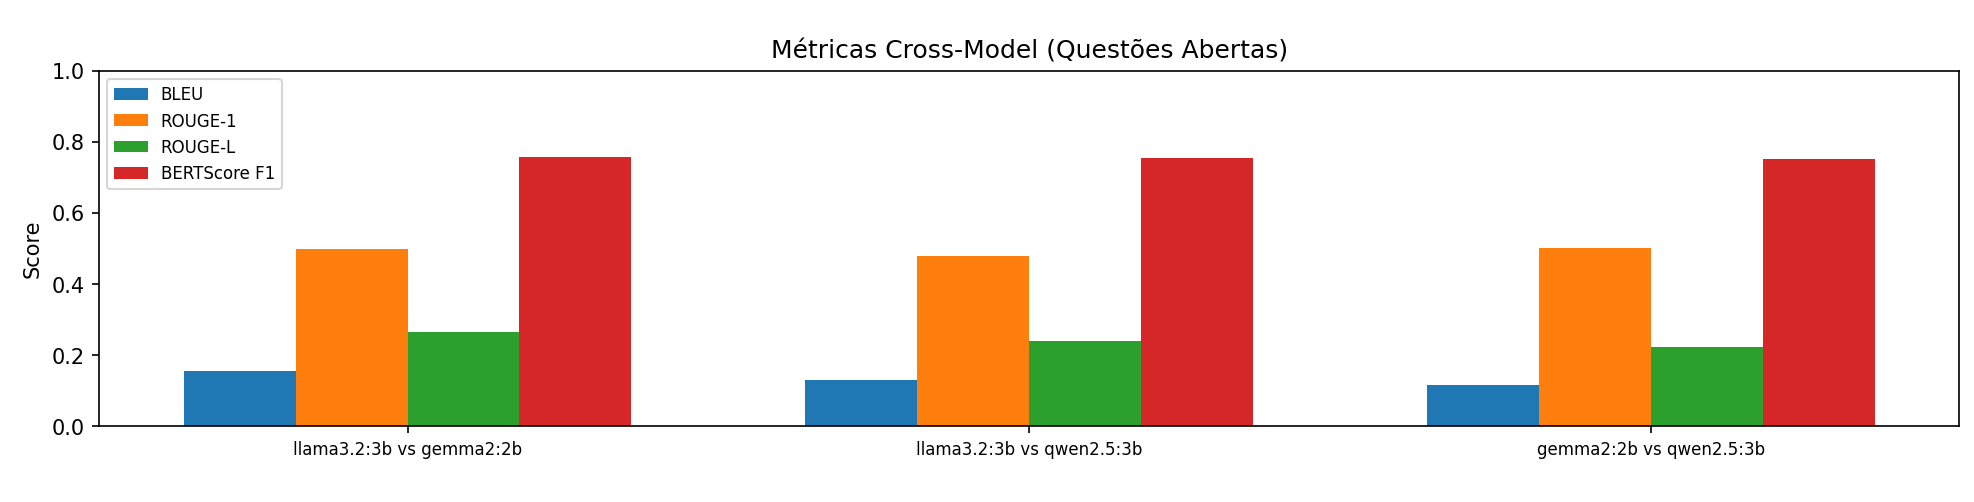
\includegraphics[width=0.85\textwidth]{images/ericles/metricas-cross-model-questoes-abertas.png}
\caption{Métricas de similaridade entre pares de modelos nas questões abertas}
\label{fig:ericles-cross-model}
\end{figure}

\subsubsection{Desempenho nas questões abertas}

A avaliação das questões dissertativas foi feita de duas formas: (i) comparação automática com a rubrica oficial do exame, e (ii) avaliação qualitativa por um modelo juiz. A Tabela~\ref{tab:ericles-rubrica} detalha o aproveitamento normalizado de cada modelo por área do Direito.

\begin{table}[H]
\centering
\caption{Aproveitamento nas questões abertas por área do Direito (\% da rubrica)}
\label{tab:ericles-rubrica}
\small
\begin{tabular}{lccc}
\toprule
\textbf{Questão} & \textbf{llama3.2:3b} & \textbf{gemma2:2b} & \textbf{qwen2.5:3b} \\
\midrule
Dir. Trabalho -- q3          & 0\%   & 0\%    & 0\%   \\
Dir. Trabalho -- q4          & 0\%   & 0\%    & 0\%   \\
Dir. Constitucional -- peça  & 100\% & --\footnotemark & 0\%   \\
Dir. Constitucional -- q1    & 0\%   & 0\%    & 0\%   \\
Dir. Constitucional -- q2    & 0\%   & 0\%    & 52\%  \\
Dir. Constitucional -- q3    & 0\%   & 0\%    & 0\%   \\
Dir. Constitucional -- q4    & 0\%   & 0\%    & 0\%   \\
Dir. Empresarial -- peça     & 0\%   & 100\%  & 0\%   \\
Dir. Empresarial -- q1       & 0\%   & 0\%    & 0\%   \\
Dir. Empresarial -- q2       & 100\% & 100\%  & 48\%  \\
Dir. Empresarial -- q3       & 100\% & 36\%   & 100\% \\
Dir. Empresarial -- q4       & 0\%   & 0\%    & 0\%   \\
\midrule
\textbf{Média}               & \textbf{25,00\%} & \textbf{21,45\%} & \textbf{16,67\%} \\
\bottomrule
\end{tabular}
\end{table}
\footnotetext{O modelo gemma2:2b não produziu uma resposta válida para esta questão.}

O resultado mais evidente é que a área de Direito do Trabalho foi um ponto cego para todos os modelos: nenhum conseguiu atender sequer parcialmente os critérios da rubrica. Em contraste, Direito Empresarial foi a área de melhor desempenho, com destaque para a questão 2 (onde llama e gemma atingiram 100\%) e a questão 3 (100\% para llama e qwen). Na área de Direito Constitucional, o llama3.2:3b se destacou ao acertar integralmente a peça profissional, enquanto o qwen2.5:3b foi o único a obter pontuação parcial na questão 2 (52\%). Nenhum modelo domina todas as questões, e os acertos de cada um se distribuem de forma complementar.

Apesar dos baixos percentuais de rubrica, a qualidade da escrita se mantém alta. A avaliação comparativa, feita por um modelo juiz (llama3.2:3b) que atribuiu notas de 0 a 5 para argumentação, precisão e coesão, mostra que o \textbf{gemma2:2b} lidera com nota final de 4,83, seguido pelo \textbf{qwen2.5:3b} (4,67) e pelo \textbf{llama3.2:3b} (3,97). O score final é calculado como $0{,}4 \times \text{argumentação} + 0{,}4 \times \text{precisão} + 0{,}2 \times \text{coesão}$. A Figura~\ref{fig:ericles-questoes-abertas} ilustra essa dualidade entre rubrica e qualidade textual.

\begin{figure}[H]
\centering
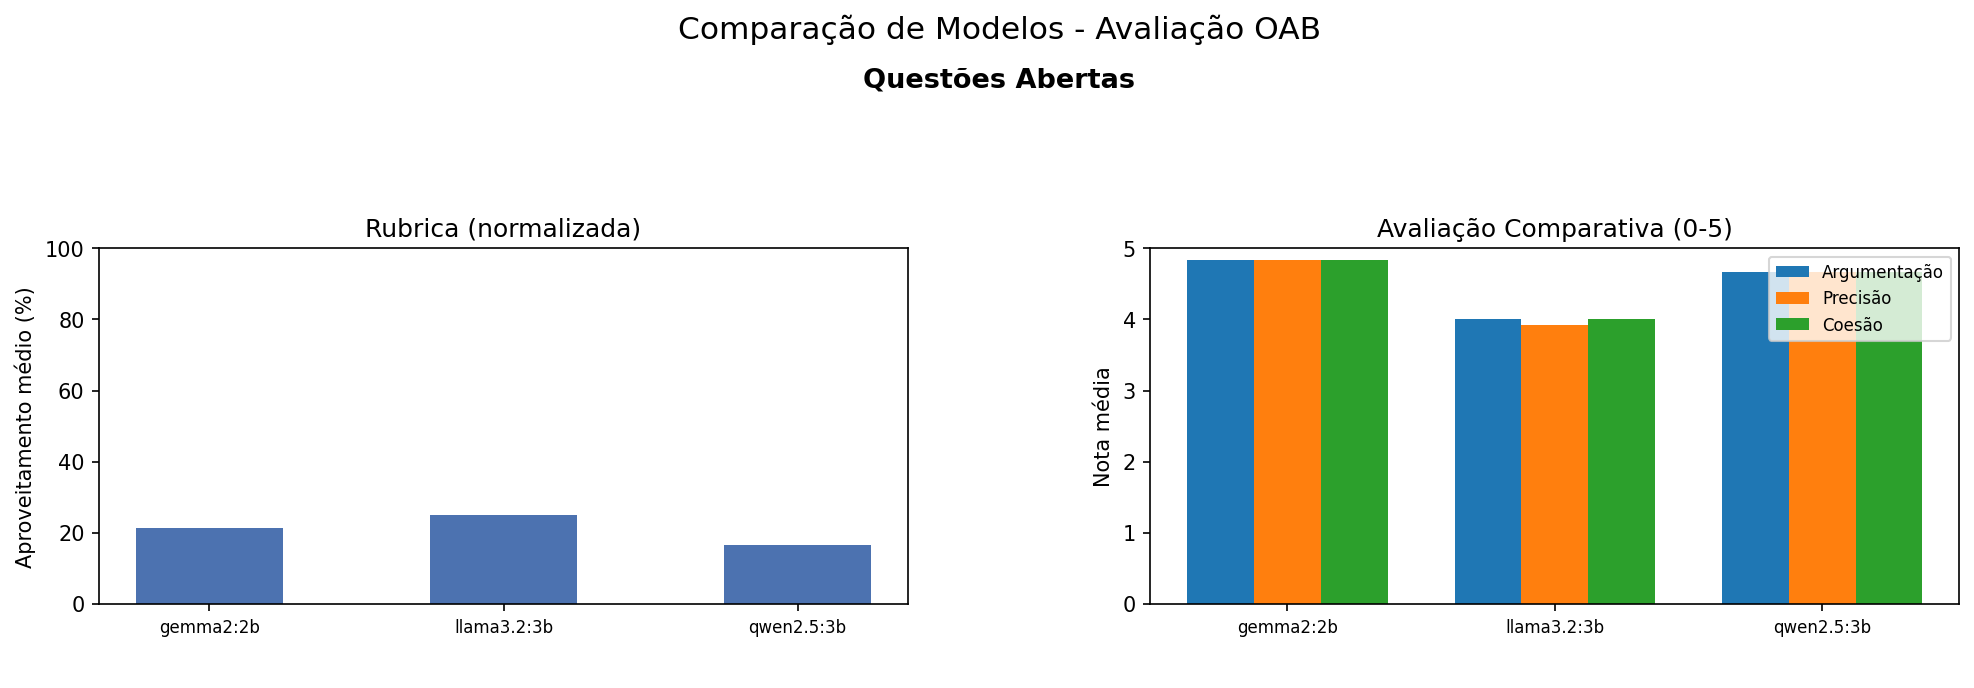
\includegraphics[width=1\textwidth]{images/ericles/questoes-abertas-comparacao-modelos.png}
\caption{Desempenho nas questões abertas: rubrica normalizada e avaliação comparativa}
\label{fig:ericles-questoes-abertas}
\end{figure}

Cabe destacar uma limitação metodológica: o modelo llama3.2:3b atua simultaneamente como avaliado e como juiz, o que pode introduzir viés de auto-preferência nas notas. Diferente de abordagens que utilizam um juiz externo (como o GPT-4o-mini), a avaliação local com o próprio modelo avaliado deve ser interpretada com cautela.

\subsubsection{Síntese e classificação final}

A Tabela~\ref{tab:ericles-leaderboard} consolida todas as métricas em uma visão geral. O ranking final depende do critério adotado: por acurácia em múltipla escolha, o qwen2.5:3b vence; por aderência à rubrica nas questões abertas, o llama3.2:3b é o melhor; e pela qualidade da escrita, o gemma2:2b se destaca.

\begin{table}[H]
\centering
\caption{Classificação consolidada dos modelos}
\label{tab:ericles-leaderboard}
\small
\setlength{\tabcolsep}{4pt}
\begin{tabular}{lcccccc}
\toprule
\textbf{Modelo} & \textbf{Acur. MC} & \textbf{Rubrica} & \textbf{Arg.} & \textbf{Prec.} & \textbf{Coesão} & \textbf{Score Final} \\
\midrule
gemma2:2b   & 40,65\% & 21,45\% & 4,83 & 4,83 & 4,83 & 4,83 \\
llama3.2:3b & 46,34\% & 25,00\% & 4,00 & 3,92 & 4,00 & 3,97 \\
qwen2.5:3b  & 50,41\% & 16,67\% & 4,67 & 4,67 & 4,67 & 4,67 \\
\bottomrule
\end{tabular}
\end{table}

Essa ausência de um vencedor absoluto reforça que avaliações baseadas em uma única métrica podem ser enganosas. O gemma2:2b, por exemplo, ficou em último lugar na acurácia de múltipla escolha (40,65\%), mas lidera com folga na qualidade de escrita (score final 4,83). Já o qwen2.5:3b tem a melhor taxa de acerto nas questões objetivas, porém obteve a menor média de rubrica nas questões abertas (16,67\%).

Em comparação com os resultados obtidos por Reinan sobre um lote distinto de questões, nota-se uma inversão no ranking de múltipla escolha: no lote de Reinan, o gemma2:2b liderou com 43,44\% de acurácia, enquanto neste lote ele ficou em último (40,65\%). Essa variação entre subconjuntos diferentes da OAB evidencia a instabilidade do desempenho desses modelos compactos, reforçando que os resultados são sensíveis à composição específica das questões avaliadas.

% ---------------------------------------------------------
\subsection{Júlia}
% ---------------------------------------------------------

\textbf{Questões atribuídas:} J1: 165--176 | J2: 1723--1845

% TODO: Adicionar contribuições individuais

% ---------------------------------------------------------
\subsection{Mikaela de Andrade Lima}
% ---------------------------------------------------------

\textbf{Questões atribuídas:} J1: 189--200 | J2: 1969--2091

% TODO: Adicionar contribuições individuais

% ---------------------------------------------------------
\subsection{Victor Leonardo Mascarenhas Soares Horta}
% ---------------------------------------------------------

\textbf{Questões atribuídas:} J1: 201--210 | J2: 2092--2210

% TODO: Adicionar contribuições individuais

% =========================================================
\section{Referências}
% =========================================================

\begin{enumerate}[nosep]
  \item Zhao, H. et al. \textit{LLM Evaluation: A Comprehensive Survey}. arXiv, 2025. Disponível em: \url{https://arxiv.org/html/2504.21202v1}.
  \item Maritaca AI. \textit{OAB Bench}. Disponível em: \url{https://github.com/maritaca-ai/oab-bench}.
  \item Garcia, E. \textit{OAB Exams}. Disponível em: \url{https://huggingface.co/datasets/eduagarcia/oab_exams}.
  \item Ollama. \textit{Ollama — Run LLMs locally}. Disponível em: \url{https://ollama.com/}.
  \item Typer. \textit{Typer — library for building CLIs in Python}. Disponível em: \url{https://typer.tiangolo.com/}.
  \item Astral. \textit{uv — Python package manager}. Disponível em: \url{https://docs.astral.sh/uv/}.
\end{enumerate}

\end{document}